\title{SAGA Tutorial Exercise \\[1em]
%\Large{SAGA Training and Tutorial Exercise } \\[1em]
\large{Ole Weidner, Hartmut Kaiser, Andre Merzky, Shantenu Jha}}

\documentclass[12pt]{article}

 \usepackage{graphicx}

\usepackage{color}
\newif\ifdraft
\drafttrue
\ifdraft
\newcommand{\amnote}[1]{   {\textcolor{magenta} { ***Andre: #1 }}}
\newcommand{\olenote}[1]{{\textcolor{blue}    { ***Ole: #1 }}}
\newcommand{\hartmutnote}[1]{  {\textcolor{green}     { ***Hartmut:    #1 }}}
\newcommand{\jhanote}[1]{  {\textcolor{red}     { ***Shantenu:    #1 }}}
 \usepackage[pdftex,colorlinks=true, linkcolor=blue,citecolor=blue,
       urlcolor=blue]{hyperref}
\else
\newcommand{\amnote}[1]{}
 \newcommand{\olenote}[1]{}
\newcommand{\note}[1]{}
\newcommand{\hartmutnote}[1]{}
 \newcommand{\jhanote}[1]{}
\fi
\begin{document}

\vspace{-1.0in}
\date{22 Nov 2010}
\maketitle

%\begin{abstract}
%This is the paper's abstract \ldots
%t\end{abstract}

\tableofcontents
\pagebreak

\section*{Scope of this Tutorial}
The scope of this tutorial is to provide the audience with the
required resources and technical knowledge (hands-on experience) to
start hacking their own distributed applications with SAGA.  We will
begin with a quick overview of how to use SAGA -- the basic, and then
quickly dive into simple yet complete applications written using
SAGA. In the latter half we will discuss a couple of ``complex''
applications, which aren't complex at all, but would have been if they
hadn't been written in SAGA.
\\
\\
\textbf{The source code for all the examples in this tutorials are part of the \textit{saga-core} source
tree and can be found at:}
\\
\\
\texttt{http://svn.cct.lsu.edu/repos/saga/core/trunk/examples/tutorial} 

\subsection{Prerequisites} This tutorial requires basic knowledge of the C/C++ programming language. Experience using the command line on a Linux/UNIX based operating system and a basic idea of what a compiler, a linker and a Makefile is might come in handy.\\[0.4em]
Unless this tutorial is going to be preceded by a SAGA installation
tutorial, the students are required to have a fully working
installation of SAGA on their laptops/lab machines (preferred), or
remote access (e.g. via SSH) to a machine with SAGA installed.
	
%\subsection*{Cheat Sheat} At the beginning of the tutorial we're going to hand out the SAGA Cheat Sheet (yet to be %created). The cheat sheet is a double-sided % (laminated, so people won't throw it away!)
%letter-sized piece of paper with hints and tips for writing, compiling, and running SAGA applications.

% \subsection{ISSGC Infrastructure}

% \begin{figure}[!ht]
%   \begin{center}
%       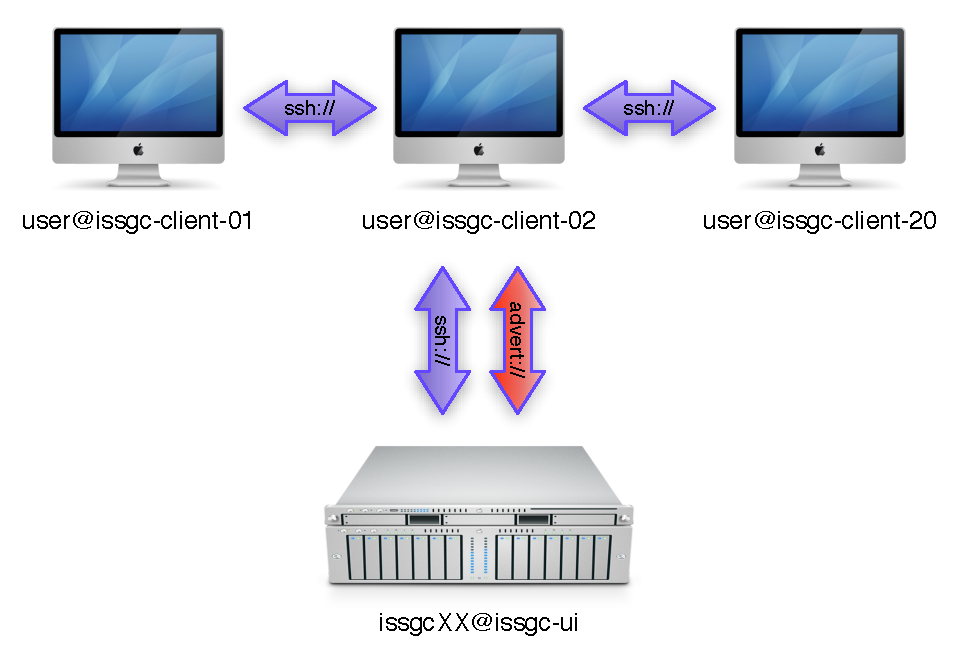
\includegraphics[width=1\textwidth]{infrastructure}
%  \end{center}
% \end{figure}

% The summer school infrastructure consists of a set of client machines issgc-client-01 to issgc-client-20 and a server issgc-ui. Since SAGA provides a uniform API for job submission, it doesn't make a difference to whether you submit your jobs through gLite, Globus, Condor or any other middleware. For the sake of simplicity, we set up the machines with SSH in a way that allows you to submit "jobs" to any other client or the server and transfer data between all available machines. Before you start using SAGA, please make sure that SSH work on your lab machine:
% \begin{verbatim}
% ssh user@issgc-client-XX /bin/hostname
% ssh issgcXX@issgc-ui /bin/hostname
% \end{verbatim}
% {\it Don't forget to assign a value to`XX''}.  Remember these host names. You will use them again in your SAGA program in the form of:
% \begin{verbatim}
% saga::url my_resource("ssh://user@issgc-client-XX");
% saga::url my_other_resource("ssh://issgcXX@issgc-ui");
% \end{verbatim}


% The server also hosts a SAGA advert DB (PostgreSQL). You will use it in one of the exercises to store some data. To make sure that you don't mess with each other's data, we created directories for each participant - make sure that you can access yours:

% \begin{center}
% \texttt{source /opt/saga-1.3.1-issgc/share/saga/saga-env.sh}
% \end{center}
% \begin{center}
%  \hspace{0.35in} \texttt{saga-advert list\_directory advert://issgc-ui//issgcXX/ ?}
% \end{center}

% Before you begin, please download the ISSGC09 student-package from our SVN sever (We recommend downloading it in /tmp/ on your machine):
% {\footnotesize
% \begin{verbatim}
% svn co https://svn.cct.lsu.edu/repos/saga-projects/tutorial/ISSGC-2009/student-package/
% \end{verbatim}}

% Also, please note the location of the Tutorial Document Servers, where we have some sample command-line utilities source code and a PDF version of a programming manual.

% \begin{center}
%   \texttt{http://issgc-server-01.polytech.unice.fr/saga/}
% \end{center}

\subsection{SAGA Applications} Every application that uses even a
single SAGA call is considered a SAGA application, since it triggers
the whole (SAGA) stack. SAGA is not a framework, but it provides the
building blocks from which to develop frameworks and/or
applications. Loosely speaking, SAGA is programming system for
distributed applications; it is important to understand that it does
not impose a specific programming model. Remember the rough taxonomy
that we presented of three ways of developing distributed applications
using SAGA: (i) Implement a distributed submission/execution mode for
a {\it legacy} application; (ii) Create a framework that supports a
specific application characteristics and/or pattern, or (iii) Compose
applications from multiple (distributed) units, which in a way makes
it an {\it a priori} application.

%Look at it as a TOOLBOX for distributed computing.
%\jhanote{Remember, we are going to use SSH adaptors for everything and nothing will USE Globus}

% \jhanote{Points/Issues to consider here: (i) Avoid Context, (ii) Copy a file given 2 URLS, and (iii) Command line Tools. Make Use of material already in the programming manual}

\subsubsection{Unit I: Command Line Utilities}
The following is a simple example of an application that copies a
file. There are more such simple (command-line utilities) that we will
discuss at: \\
\texttt{https://svn.cct.lsu.edu/repos/saga/core/trunk/tools/clutils/}

%\jhanote{Both the location above and the URL below needs updating}

\begin{verbatim}
///////////////////////////////////////////////////////////////////////////////
#include <saga/saga.hpp>

int main(int argc, char * argv[]) 
{
  saga::url source("ssh://hostname//etc/passwd"); 
  saga::url target(".");
  
  saga::filesystem::file file (source, saga::filesystem::Read);
  file.copy(target);

  return 0;
}
///////////////////////////////////////////////////////////////////////////////
\end{verbatim}

% \jhanote{Ole: I guess this is where we take a diversion into ``clutils'' and ``shell''. I have put the slide into tutorial/ISSGC-2009/student-package/slides
% Maybe we should now put the code for clutils and shell into
% tutorial/ISSGC-2009/student-package/tools/}

% {\footnotesize
% \begin{verbatim}
% svn co https://svn.cct.lsu.edu/repos/saga/tags/saga-1.3.1-issgc-release/tools/ 
% \end{verbatim}}

{\it Q: Which of the three types of distributed applications would you
  classify the above copy program into?}

\subsubsection{Unit II} \textbf{Compiling and linking.} Like
with any other C/C++ library, you have to let the compiler and the
linker know where to find the header files and the library. To make
life easier, SAGA provides a Makefile which you can include in order
to build your application:

\begin{verbatim}
SAGA_SRC          = $(wildcard *.cpp) 
SAGA_ADD_BIN_OBJ  = $(SAGA_SRC:%.cpp=%.o) 
SAGA_BIN          = my_saga_app 

include $(SAGA_LOCATION)/share/saga/make/saga.application.mk 

## Other (optional) compiler and linker flags 
SAGA_CPPFLAGS    += -I/opt/super/include 
SAGA_LDFLAGS     += -L/opt/super/lib -lsuper 
\end{verbatim}

Of course it is also possible to compile and link a SAGA application manually:

\begin{verbatim}
g++ -Wall -I$SAGA_LOCATION/include -pthread \ 
    -L$SAGA_LOCATION/lib \
    -lsaga_engine -lsaga_package_job -lsaga_package_XYZ \
    <FILENAME>.cpp

\end{verbatim}

\subsubsection{Unit III: Running a SAGA application.} 

SAGA needs to know where its configuration files are located and
where to find its middleware adaptors. This is done via the
\texttt{SAGA\_LOCATION} environment variable, e.g.: 

\begin{verbatim}
export SAGA_LOCATION=/opt/saga-1.5.3-pre/
\end{verbatim}

In order to run a SAGA application, you have to make sure that all
required libraries can be found by the loader in case SAGA is not 
installed within the default system path. The easiest way to do
that is to set the LD\_LIBRARY\_PATH (DYLD\_LIBRARY\_PATH on Mac OS), e.g.:

%\jhanote{Fix the LD\_LIBRARY\_PATH below. Make Generic}

\begin{verbatim}
export LD_LIBRARY_PATH=$SAGA_LOCATION/lib:$LD_LIBRARY_PATH
\end{verbatim}

%\jhanote{Need to fix here too..}

%On the lab machines (issgc-client-XX) you can source your environment
%conveniently by typing:

%\begin{verbatim}
%source /opt/saga-1.3.1-issgc/share/saga/saga-env.sh
%\end{verbatim}

Another (optional) environment variable that might come in handy is
\texttt{SAGA\_VERBOSE} in case something goes wrong. If set, SAGA will
print detailed debug information to a log-file in the working directory, e.g.:

\begin{verbatim}
export SAGA_VERBOSE=100
\end{verbatim}


\subsubsection{Unit IV: SAGA-based Applications:}

You have had some initial exposure to the API when going through the
command-line utilities.  In this section, we will work with three
different examples. The aim of these applications is to give you a
quick feel for how SAGA is actually utilized to develop {\it complete,
  stand-alone} distributed applications. And although these examples
are by necessity very simple, they are representative of the way you
would use SAGA in actual real-world examples to develop many of the
scientific applications.

%  you heard about in today's lecture such as
% Replica-Exchange and C0$_2$ Sequestration problem(s).

In the first example, we will introduce a simple ``Hello Distributed
World!'', where the aim will be to submit three simple remote jobs
using SAGA. In the second example application
(``chaining\_jobs.cpp''), we will serialize the launch of three
(remote) jobs, so that the second job is launched after the first, and
the third job is launched after the second. In the third example
application (``depending\_jobs.cpp''), we will start an application
that once started, is able to re-spawn itself on another machine, and
after doing so increments a ``global counter''. Finally, we will leave
you with a programming exercise that will build upon your
understanding of application examples 2 and 3.

\pagebreak
\subsection{Example 1: Hello distributed world! \\
(\texttt{hello\_world.cpp})} Submit three jobs to
three machines. One returns �Hello�, one returns �Distributed� and one
returns �World�. They may or may not return in the right order. This
should give you an an idea how they could potentially speed up their
application using multiple resources. Also, execute the program
several times. Do you notice any difference in the outputs? Are they
same?

\begin{verbatim}
///////////////////////////////////////////////////////////////////////////////
#include <iostream>
#include <saga/saga.hpp>
#include <boost/thread.hpp>

///////////////////////////////////////////////////////////////////////////////
// The hello_world example is meant to be a very simple and first example to 
// try when it comes to SAGA. It's purpose is to spawn 3 (possibly remote) 
// identical jobs (/bin/echo) while passing the 3 words "Hello", "distributed", 
// and "world!" on their command lines. The result is that the jobs will print
// the respective command line arguments (hey, it's /bin/echo we're 
// launching...). The master job (this one) waits for the 3 child jobs to 
// finish. It intercepts the generated output and prints it to the user.
//
// Depending on which child jobs finish first the overall printed message might
// be some combination of the 3 arguments we passed. But most of the time you
// will see "Hello distributed world!", which is our way of saying hello and
// welcome to the world of SAGA.
///////////////////////////////////////////////////////////////////////////////


///////////////////////////////////////////////////////////////////////////////
// The URLs to spawn jobs to.  Please change the 3 macros below to the URLs 
// you want the 3 childs to be spawned to.
///////////////////////////////////////////////////////////////////////////////
#define URL1 "fork://localhost"
#define URL2 "fork://localhost"
#define URL3 "fork://localhost"



///////////////////////////////////////////////////////////////////////////////
// the routine spawning the SAGA jobs and waiting for their results
void run_a_job(saga::url url, std::string argument)
{
    try {
        saga::job::service js (url);
        saga::job::ostream in;
        saga::job::istream out;
        saga::job::istream err;

        // run the job
        saga::job::job j = js.run_job("/bin/echo " + argument, "", in, out, err);

        // wait for the job to finish
        j.wait ();

        // if the job finished successfully, print the generated output
        if (j.get_state () == saga::job::Done) 
        {
            std::string line;
            while (!std::getline(out, line).eof())
                std::cout << line << '\n';
        }
        else {
            std::cerr << "SAGA job: " << j.get_job_id() << " failed\n";
        }
    }
   catch (saga::exception const& e) {
        std::cerr << "saga::exception caught: " << e.what () << std::endl;
    }
    catch (std::exception const& e) {
        std::cerr << "std::exception caught: " << e.what () << std::endl;
    }
    catch (...) {
        std::cerr << "unexpected exception caught" << std::endl;
    }
}

///////////////////////////////////////////////////////////////////////////////
int main(int argc, char* argv[])
{
    // run 3 separate threads executing the saga calls
    boost::thread t1 (run_a_job, URL1, "Hello");
    boost::thread t2 (run_a_job, URL2, "distributed");
    boost::thread t3 (run_a_job, URL3, "world!");

    // wait for all spawned threads to finish
    t1.join();
    t2.join();
    t3.join();
    return 0;
}
///////////////////////////////////////////////////////////////////////////////
\end{verbatim}

\pagebreak
\subsection{Example 2: Multiple Sequential Jobs \\
(\texttt{chaining\_jobs.cpp})}
\textbf{Applications} The aim of this section is to see how SAGA is
used to implement common {\it higher-level} functionality that is used
by Distributed Applications (DA). Specifically, we will look at two
commonly occurring functionality required by DA.

{\bf Example 1:} Here we will demonstrate the ability to checkpoint,
use a specified resource, self-migrate and restart on a different
computational resource. 

%There are multiple reasons this might be required. % (see lecture notes)
Here we will demonstrate this capability using the \textbf{Hello
  distributed world!} example discussed in Unit IV.  Instead of
launching three jobs on three machines, we will launch one job on one
machine, which will then launch itself on another machine, which in
turn will do so onto yet another machine.


\begin{verbatim}
///////////////////////////////////////////////////////////////////////////////
#include <iostream>
#include <saga/saga.hpp>

///////////////////////////////////////////////////////////////////////////////
// The chaining_jobs example tries to overcome one of the limitations of the 
// hello_world example: it introduces dependencies between 3 (possibly remotely)
// spawned childs. In this example the next child will be spawned only after 
// the previous one has finished its execution. To make it more interesting we 
// now use /usr/bin/bc to do some calculations, where the result of the previous
// calculation is used as the input for the next one.
//
// Try to make more complex calculations if you like!
///////////////////////////////////////////////////////////////////////////////

///////////////////////////////////////////////////////////////////////////////
// The URLs names to spawn jobs to.  Please change the 3 macros below to the 
// urls you want the 3 childs to be spawned to.
///////////////////////////////////////////////////////////////////////////////
#define URL1 "fork://localhost"
#define URL2 "fork://localhost"
#define URL3 "fork://localhost"

///////////////////////////////////////////////////////////////////////////////
// the routine spawning the SAGA jobs and waiting for their results
std::string increment (saga::url url, std::string argument)
{
    try {
        saga::job::service js (url);
        saga::job::ostream in;
        saga::job::istream out, err;

        // run the job
            s = j.get_state();

        // if the job didn't start successfully, print error message
        if ( j.get_state () != saga::job::Running ) {
            std::cerr << "SAGA job: " << j.get_job_id() << " failed" << std::endl;
            return argument;
        }

        // feed the remote process some input, receive result, 
        // and quit remote process
        in << "1 + " << argument << std::endl;
        std::string line;
        std::getline (out, line);
        in << "quit\n";

        return line;
    }
    catch (saga::exception const& e) {
        std::cerr << "saga::exception caught: " << e.what () << std::endl;
    }
    catch (std::exception const& e) {
        std::cerr << "std::exception caught: " << e.what () << std::endl;
    }
    catch (...) {
        std::cerr << "unexpected exception caught" << std::endl;
    }
    return argument;    // by default just return argument
}

///////////////////////////////////////////////////////////////////////////////
int main(int argc, char* argv[])
{
    std::string result;

    // run the incrementor 3 times (i.e. spawn 3 jobs to increment the counter)
    result = increment (URL1, "1");
    result = increment (URL2, result);
    result = increment (URL3, result);

    std::cout << "The overall result is: " << result << std::endl;

    return 0;
}
///////////////////////////////////////////////////////////////////////////////
\end{verbatim}

Once developed, this capability can be utilized by a wide range of
different applications. In other words this capability described/shown
above is independent of any specific application logic. Do you know of
a (Scientific) application that could utilize this feature?

\newpage

\subsection{Example 3: Managing Dependencies between Jobs \\
(\texttt{depending\_jobs.cpp})}

In this example, we will introduce the {\it advert service} as a
simple mechanism to provide coordination between different distributed
tasks.  Specifically, the advert service will be used by a set of jobs
to increment a global counter everytime a job is successfully
spawned. There are other ways of {\it coordinating} distributed
tasks/jobs, but the idea of a centralized data-store is arguably the
simplest, even if not the most robust (fault-tolerant) or tuned for
performance. Also, of interest is the \texttt{respawn} method.

%This application is executed using the following command in the sub-directory 
%student-package/sourcecode from where you checked out the code from SVN.

%\jhanote{This URL needs updating}

%{\footnotesize
%\begin{verbatim}
%user@issgc-client-10:/tmp/student-package/sourcecode$

%saga-advert remove_entry advert://issgc-ui//issgcXX/result_ex_2
%./depending_job ssh://user@134.59.140.163 ssh://user@134.59.140.164
%saga-advert retrieve_string advert://issgc-ui//issgcXX/result_ex_2
%\end{verbatim}}

\begin{verbatim}
///////////////////////////////////////////////////////////////////////////////
#include <iostream>
#include <cassert>
#include <saga/saga.hpp>
#include <boost/lexical_cast.hpp>

///////////////////////////////////////////////////////////////////////////////
//
// Start this example by providing an arbitrary number of URLs on the command 
// line. It will re-spawn itself to each of the URLs. Each instance will 
// increment a number stored in a central counter store, using the advert service.
//
//
// example usage (slightly shortened):
//
//   # saga-advert remove_entry /tutorial/depending_jobs/counter
//
//   # saga-advert dump_directory /tutorial/depending_jobs/
//     /tutorial/depending_jobs/
//
//   # make && ./depending_jobs fork://localhost fork://localhost
//   advert entry does not yet exist - initialize counter to 0
//
//   # saga-advert dump_directory /tutorial/depending_jobs/
//     /tutorial/depending_jobs/
//         /tutorial/depending_jobs/counter
//           value     	: 2
//
//   # make && ./depending_jobs fork://localhost fork://localhost
//
//   # saga-advert dump_directory /tutorial/depending_jobs/
//     /tutorial/depending_jobs/
//         /tutorial/depending_jobs/counter
//           value     	: 4
//
///////////////////////////////////////////////////////////////////////////////
#define RESULT_STORE  "/tutorial/depending_jobs/counter"  // advert to store counter to
#define JOB_PATH      "./depending_jobs"                  // put the correct path here

///////////////////////////////////////////////////////////////////////////////
// retrieve the current value from the advert (counter store)
bool get_counter(int& counter)
{
    counter = 0;
    try {
        saga::advert::entry e (RESULT_STORE, saga::advert::Read);
        counter = boost::lexical_cast <int> (e.get_attribute ("value"));
    }
    catch (saga::does_not_exist const& e) {
        std::cout << "advert not existing - init counter to 0" << std::endl;
        counter = 0;
        return true;
    }
    catch (saga::exception const& e) {
        std::cerr << "saga::exception caught: " << e.what () << std::endl;
        return false;
    }
    catch (std::exception const& e) {
        std::cerr << "std::exception caught: " << e.what () << std::endl;
        return false;
    }
    catch (...) {
        std::cerr << "unexpected exception caught" << std::endl;
        return false;
    }
    return true;
}

///////////////////////////////////////////////////////////////////////////////
// store the current value into the advert (counter store)
bool set_counter(int counter)
{
    try {
        saga::advert::entry e(RESULT_STORE, 
                              saga::advert::CreateParents | 
                              saga::advert::Create        | 
                              saga::advert::ReadWrite     );
        e.set_attribute ("value", boost::lexical_cast <std::string> (counter));
    }
    catch (saga::exception const& e) {
        std::cerr << "saga::exception caught: " << e.what () << std::endl;
        return false;
    }
    catch (std::exception const& e) {
        std::cerr << "std::exception caught: " << e.what () << std::endl;
        return false;
    }
    catch (...) {
        std::cerr << "unexpected exception caught" << std::endl;
        return false;
    }
    return true;
}

///////////////////////////////////////////////////////////////////////////////
// the routine spawning the SAGA jobs and waiting for their counter
void respawn(int argc, char *argv[])
{
    assert(argc > 1);     // we shouldn't end up here without any given URL
    try 
    {
        // start the johb server on the given URL   
        saga::url url (argv[1]);
        saga::job::service js (url);

        // compose the command line, skip first argument
        std::string commandline (JOB_PATH);
        for (int i = 2; i < argc; ++i) {
            commandline += " ";
            commandline += argv[i];
        }

        // run the job 
        saga::job::job j = js.run_job(commandline);

        // wait for the job to start
        saga::job::state s = j.get_state();
        while (s != saga::job::Running && s != saga::job::Failed)
            s = j.get_state();

        // if the job didn't start successfully, print error message
        if (s == saga::job::Failed) {
            std::cerr << "SAGA job: " << j.get_job_id() << " failed (state: " 
                      << saga::job::detail::get_state_name(s) << ")\n";
        }

        // wait for the job to Finish
        s = j.get_state();
        while (s == saga::job::Running)
            s = j.get_state();
    }
    catch (saga::exception const& e) {
        std::cerr << "saga::exception caught: " << e.what () << std::endl;
    }
    catch (std::exception const& e) {
        std::cerr << "std::exception caught: " << e.what () << std::endl;
    }
    catch (...) {
        std::cerr << "unexpected exception caught" << std::endl;
    }
}
///////////////////////////////////////////////////////////////////////////////
\end{verbatim}

  \noindent Not surprisingly the code snippet above is independent of
  any application specific details and focuses on the assignment of
  workloads to workers, execution and then retrieval. This specific
  approach adopted here relies heavily on the use of the Advert
  Service.

\begin{verbatim}
///////////////////////////////////////////////////////////////////////////////
int main(int argc, char* argv[])
{
    if (argc == 1) {
        // no more URLs are given, we're done!
        int counter = 0;
        if (get_counter(counter))
            std::cout << "The overall counter is: " << counter << std::endl;
    }
    else {
    // otherwise get current value, increment it, and store new value
        int counter = 0;
        get_counter (counter);   // will set counter to zero initially

        // re-spawn this job, increment counter
        // if set_counter fails, don't bother to respawn
        if (set_counter(counter + 1)) 
            respawn(argc, argv);
    }

    return 0;
}
///////////////////////////////////////////////////////////////////////////////
\end{verbatim}

\noindent {\it Q: Can you think of an a usage-mode that can be supported by the general functionality to respawn a job? Long-running Simulations? What else?}

\pagebreak
\subsection{Additional Real World Example} 
\noindent % The requirement of coordination of distributed, often
% heterogeneous units is a fundamental {\it vector} of distributed
% applications. (See Lecture Notes).
We will briefly discuss MapReduce -- a computational pattern made
famous by Google's use for its Search Engine Infrastructure.  The
fundamental idea is that there is a Master which coordinates the
distribution of work to a large number of Workers, and manages the
merging of the output of the computation that the Workers produce. In
addition to performance, a fundamental challenge is the need to be
able to coordinate Master-Workers across a wide range of distributed
systems. For more details, check out the code at:

\begin{verbatim}
https://svn.cct.lsu.edu/repos/saga-projects/applications/MapReduce/
\end{verbatim}

\pagebreak

\subsection{Programming Exercise:} 

\subsubsection{Exercise 1:} Recall how when the program hello\_world
was executed the order of the values returned often varied. Can you
use introduce dependencies between the jobs so as to ensure that the
output is always in order ``Hello Distributed World!''?

\subsubsection{Exercise 2:} In earlier examples, we introduced the
underlying concepts of submitting jobs and coordination amongst
multiple distributed jobs (tasks), where we updated the value of a
counter. Can the same approach (i.e. advert) be used to coordinate the
submission of multiple jobs? In effect, this is a way of informing a
job (that is ready to spawn another job) about which (possible)
machines to spawn too.  The aim of this exercise is for you to
complete the code by implementing some (i) job submission
functionality, and (ii) accessing advert entries.  (We will post a
sample solution to this at the end of the tutorial).

\begin{verbatim}
<CODE>
\end{verbatim}

Think of generalizations to this concept: Say one application is
``producing'' this information (that is a list of possible resources),
and this information is being ``consumed'' by another application.

\subsection{Conclusion}

Let us recap that there are multiple types of distributed
applications. What you have seen here are simple applications that
utilize distributed functionality, such as remote job submission to
achieve tasks.  What you should take away from this tutorial are
essentially the following:

\begin{itemize}

\item Distributed Applications can be developed much like regular
  applications.  The challenges facing Distributed Applications --
  development and deployment are different from traditional
  applications and many of those challenges arise from the distributed
  infrastructure. It is to precisely meet these ``unique'' distributed
  computing challenges that there is a need for simple, standard and
  pervasive application level interface such as SAGA was conceived.

\item We have focused on some of the challenges of developing
  distributed applications, such as coordinating distributed tasks. We
  have shown the ability to do so in a simple fashion; however this is
  not necessarily scalable, and poses challenges for many real-world
  applications. Some other real-world challenges we have not discussed
  here are fault-tolerance, recovery, replication etc. SAGA provides
  APIs to these ``Advanced'' features as well.

\item Interestingly, we have built all the distributed functionality
  around simple ``ssh'' adaptors; if you wanted to launch to a Globus
  or a Condor specific infrastructure, you would just configure SAGA
  to utilize Globus or Condor specific adaptors.

\item Remember the following website \texttt{http://saga.cct.lsu.edu}
  is your source of information for all things SAGA. And this document
  can be found at:

%\jhanote{Fix URLs}

%{\footnotesize
%\begin{verbatim}
% https://svn.cct.lsu.edu/repos/saga-projects/tutorial/ISSGC-2009/
%\end{verbatim}}

\end{itemize}
\end{document}

